\documentclass[10pt, margin=1mm]{standalone}
\usepackage{tikz}
\usetikzlibrary{arrows,decorations.pathmorphing,backgrounds,positioning,fit,petri,shapes}
\pgfdeclarelayer{bg}    % declare background layer
\pgfsetlayers{bg,main}  % set the order of the layers (main is the standard layer)
\usepackage{graphicx}
\usepackage{amsmath,amssymb,amsfonts}
\usepackage{fontawesome}

\definecolor{myblue}{RGB}{76,114,176}
\definecolor{myorange}{RGB}{221,132,82}

\usetikzlibrary{shapes.multipart}

\begin{document}
    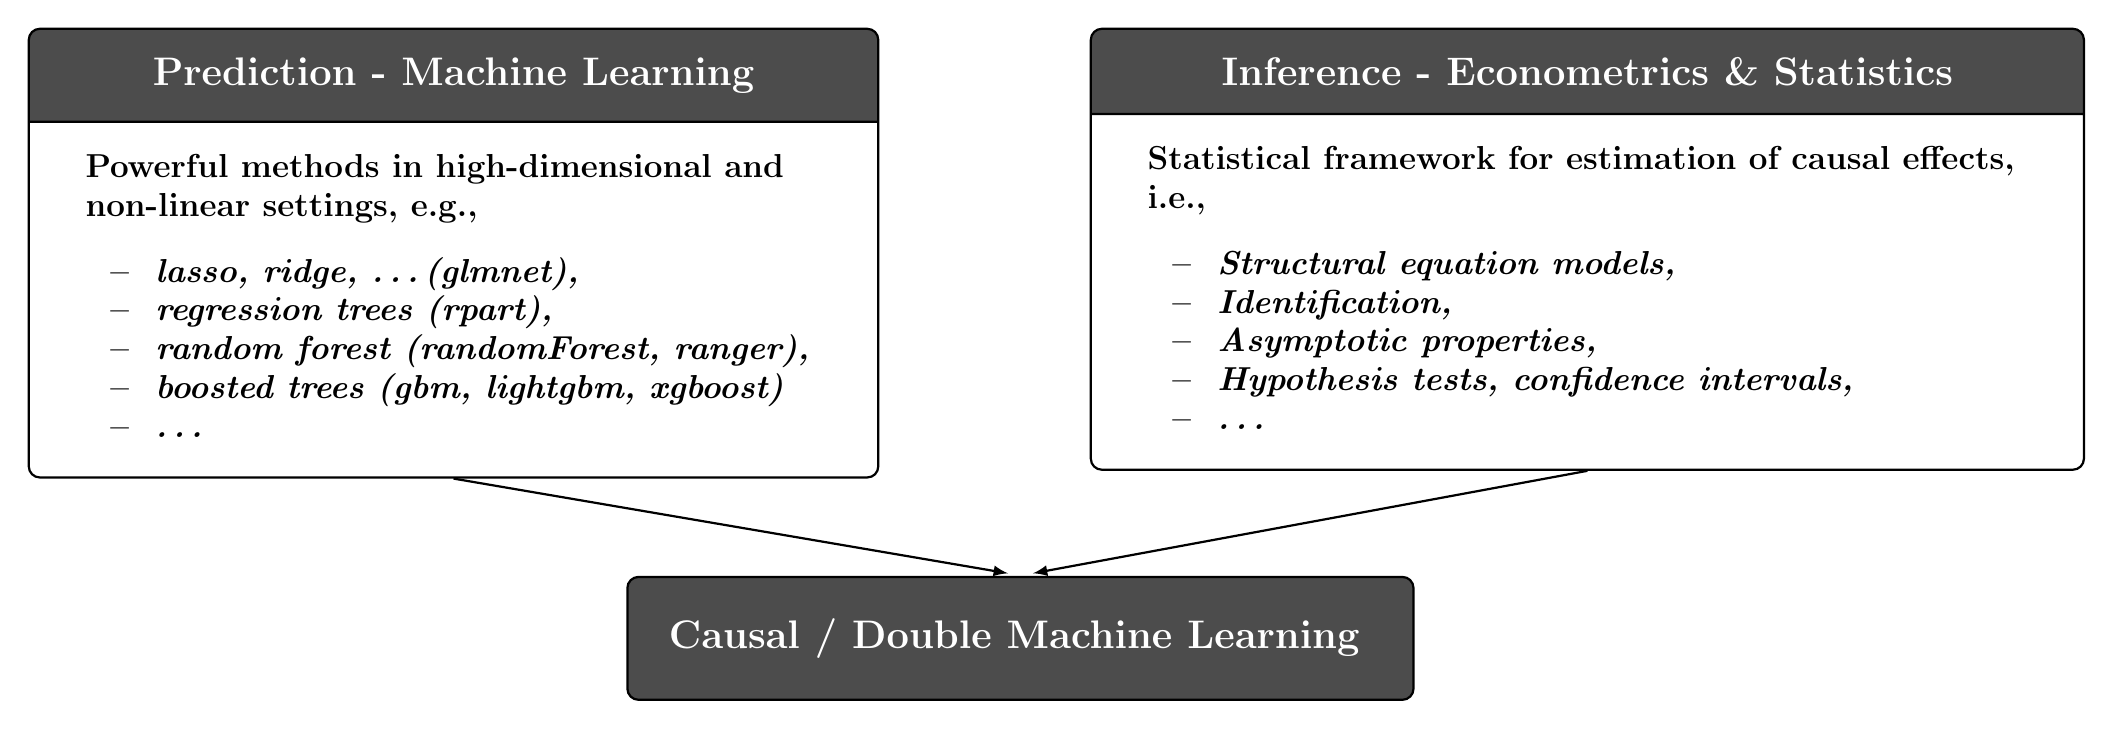
\begin{tikzpicture}[scale=0.9]
%[auto,scale=1,transition/.style={rectangle,draw=black!50,thick,
%inner sep=5pt,minimum width=8cm,minimum height=1cm,font=\large,text width=8cm}]
\tikzstyle{every node}=[font=\large\bf]

\node[thick,below,
minimum width=7cm,
rectangle split,rectangle split parts=2, inner sep=10pt, rounded corners, draw=black,
rectangle split part align={center, left},
rectangle split part fill={black!70, white}] at (-8, 0) (ml) {
\textcolor{white}{
{\Large Prediction - Machine Learning}}
\nodepart{two}{%
{
\begin{tabular}{l}
Powerful methods in high-dimensional and \\
non-linear settings, e.g.,\\
\\[-0.8ex]
\text{ } -- \textit{ lasso, ridge, \ldots (glmnet),} \\
\text{ } -- \textit{ regression trees (rpart),}\\
\text{ } -- \textit{ random forest (randomForest, ranger),}\\
\text{ } -- \textit{ boosted trees (gbm, lightgbm, xgboost)}\\
\text{ } -- \textit{ \ldots}
\end{tabular}
}
}
};

\node[thick,below,
minimum width=7cm,
rectangle split,rectangle split parts=2, inner sep=10pt, rounded corners, draw=black,
rectangle split part align={center, left},
rectangle split part fill={black!70, white}] at (8, 0) (econ) {
\textcolor{white}{
{\Large Inference - Econometrics \& Statistics}}
\nodepart{two}{%
{
\begin{tabular}{l}
Statistical framework for estimation of causal effects,\\ i.e., \\\\[-0.8ex]
\text{ } -- \textit{ Structural equation models,} \\
\text{ } -- \textit{ Identification,}\\
\text{ } -- \textit{ Asymptotic properties,}\\
\text{ } -- \textit{ Hypothesis tests, confidence intervals,}\\
\text{ } -- \textit{ \ldots}
\end{tabular}
}
}
};


\node[anchor=north, thick,above, fill=black!70, align=center,
rectangle, inner sep=15pt, rounded corners, draw=black] at (0, -9.5) (dml) {
{\Large \textcolor{white}{Causal / Double Machine Learning}}
};

\draw[-latex, thick] (ml.south) -- ([xshift=-5pt, yshift=1pt]dml.north);
\draw[-latex, thick] (econ.south) -- ([xshift=5pt, yshift=1pt]dml.north);

\end{tikzpicture}

\end{document}
